\section{连接数可扩放的 RDMA 网卡实现}
\label{socksdirect:sec:discussion}


\begin{figure}[htbp]
	\centering
	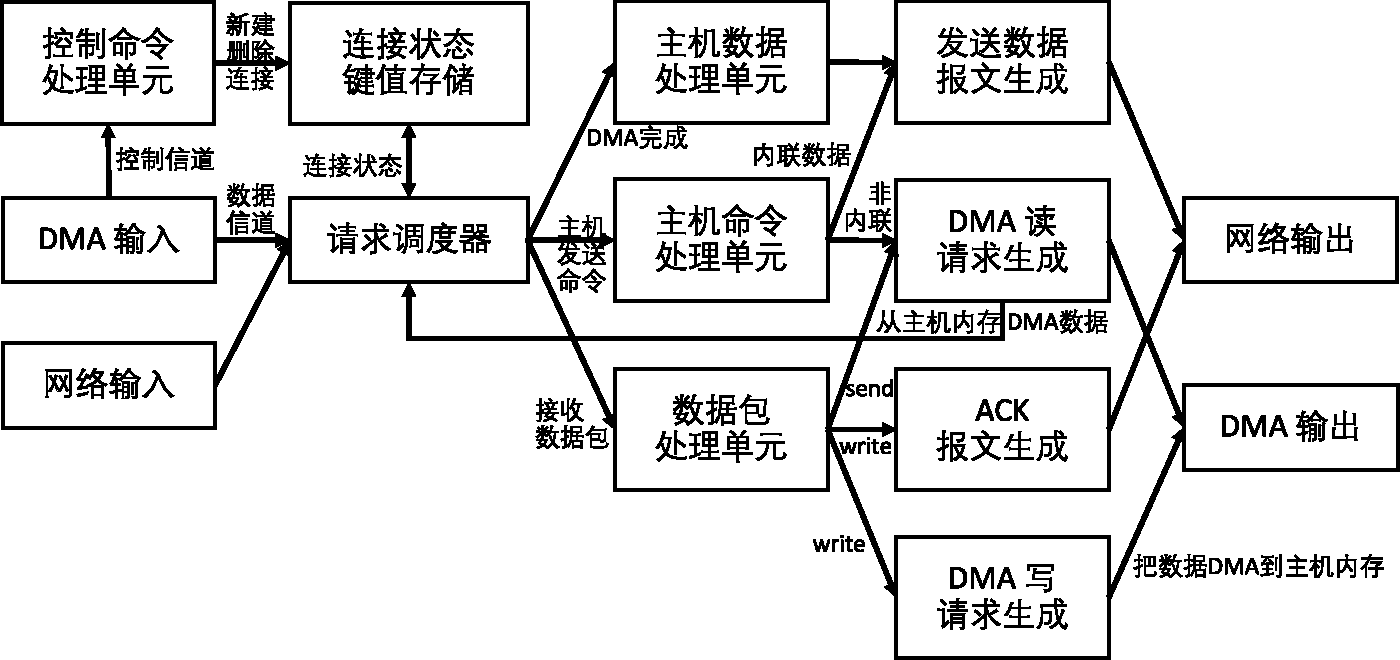
\includegraphics[width=0.9\textwidth]{images/scalable_rdma.pdf}	
	\caption{基于可编程网卡的连接数可扩放 RDMA。}
	\label{socksdirect:fig:scalable-rdma}
\end{figure}

%\textbf{Communicating with TCP/IP peers.}
%We use a user-space networking stack to communicate with regular TCP/IP peers, but the compatibility may be limited~\cite{yasukata2016stackmap}.
%To solve this problem, after receiving the TCP SYN+ACK, the monitor can create an established kernel TCP connection using TCP connection repair~\cite{tcp-connection-repair}.
%Moreover, if the application and monitor share a network namespace, the monitor can send the kernel 文件描述符 to the application via Unix domain socket, then \libipc{} can use the 文件描述符 without delegation to the monitor.

%\textbf{Connecting to many RDMA capable hosts.}
%With a lot of hosts, the 网卡 still suffer from performance degradation due to large number of connections.
%In contrast, user-space networking stack alleviates this problem because the 网卡 is stateless.
%We provide a socket option to enable applications to delegate operations to the monitor and use user-space networking stack even if the peer supports RDMA.
%An application can choose to use RDMA for latency sensitive and throughput demanding connections, and user-space networking stack for others.

\parab {扩放到大量连接。}
\sys {}对许多连接的可伸缩性受共享内存和RDMA的限制。
为了表明 \libipc {} 和监视器不是瓶颈,本节在两个重用RDMA QP和共享内存的进程之间创建了很多连接。使用 \libipc {} 的应用程序线程每秒可以创建1.4~M个新连接,这是Linux的20倍和mTCP的2倍 \cite {jeong2014mtcp}。监视器每秒可以创建5.3~M个连接。

由于主机内的进程数量有限,因此SHM连接的数量可能不会很大。
但是,一台主机可能连接到许多其他主机,RDMA的可扩展性成为一个问题。
这归结为两个问题。
首先,RDMA 网卡使用网卡内存作为缓存来保持每个连接状态。有数千个并发连接,性能受到频繁缓存未命中的影响 \cite {mprdma,kaminsky2016design,kalia2018datacenter}。
但是,网卡配备了小内存,因为RDMA传统上部署在中小型集群中。
随着近年来大规模的RDMA部署 \cite {guo2016rdma},商品网卡拥有更大的内存来存储数千个连接 \cite {kalia2018datacenter}而Smart网卡拥有千兆字节的DRAM~ \cite {mellanox-innova,mellanox-bluefield,smartnic}。
因此,我们预测未来的数据中心不会为网卡缓存未命中问题担心过多。
第二个问题是本文的测试平台中建立RDMA连接需要大约 $30 \mu s$,这对于短连接很重要。但是,此过程仅涉及本地CPU和网卡之间的通信,希望未来的工作能够得到改进。

%Another promising direction to solve the RDMA concurrency issue is to implement the reliable transport in CPU, and the 网卡 remains stateless. However, RDMA UD does not support one-sided write, so the ring buffer in Sec.~\ref{socksdirect:subsec:lockless-queue} will not work. Existing software RDMA~\cite{soft-roce} has low performance. It would be interesting to co-design software and 网卡.

\textbf {RDMA的QoS。}
将数据平面性能隔离和拥塞控制卸载到 RDMA 网卡上是一个越来越流行的研究方向 \cite {peter2016arrakis,zhu2015congestion,lu2017memory,mprdma,mittal2018revisiting},因为数据中心的网卡正变得越来越可编程  \cite{smartnic,cavium,kaufmann2015flexnic,mellanox-innova,mellanox-bluefield},而公有云已经在虚拟机之外的网络功能中提供了 QoS \cite {li2016clicknp,panda2016netbricks,floem-osdi18}。

%\textbf{Networking stack on other layers.}
%RDMA: lower layer,
%eRPC, message queue, etc: higher layer.

%\section{Related Work}
%\label{socksdirect:sec:related-work}

%Several mostly related works have been discussed in Sec.~\ref{socksdirect:subsec:related-work}.

\iffalse
\parab{Linux kernel optimization.}
One line of research optimizes the kernel stack for higher socket performance. FastSocket~\cite{lin2016scalable} and Affinity-Accept~\cite{pesterev2012improving} scale connection creation to multiple cores, but synchronization is still needed when multiple threads share a socket.
FlexSC~\cite{soares2010flexsc} proposes exception-less system calls to reduce kernel crossing overhead.
Zero-copy socket~\cite{thadani1995efficient,chu1996zero} still needs copy-on-write on senders.
In addition, they fail to remove cache miss and transport overheads.


\parab{New OS stacks.}
Another line of research proposes new OS stacks with modified socket interface, mostly aiming at zero copy and fast event notification. Existing socket applications need modifications to use the new interfaces.
For intra-server connections, Arrakis~\cite{peter2016arrakis} and IX~\cite{belay2017ix} use the 网卡 to forward packets from one process to another. The hairpin latency from CPU to 网卡 is at least two PCIe delays, which is one order of magnitude higher than inter-core cache migration delay. In addition, the data plane switching throughput of a 网卡 is constrained by PCIe bandwidth (Figure~\ref{socksdirect:fig:eval-corenum-tput}).

For inter-server connections, most OS stacks implement transport in software. IX~\cite{belay2017ix} and Stackmap~\cite{yasukata2016stackmap} run in the kernel to enforce QoS policy or preserve protocol compatibility with Linux, while Arrakis~\cite{peter2016arrakis} and SandStorm~\cite{marinos2014network} run in user mode to maximize performance.
RDMA and transport virtualization~\cite{tsai2017lite,niu2017network} also enforce QoS in the hypervisor.
Due to the additional level of indirection, kernel stacks cannot remove kernel crossing, while batched syscalls add latency.
Further, large-scale deployment of kernel-based stacks is more complicated than user-space libraries~\cite{andromeda}.
\sys offloads transport and QoS to 网卡 hardware.
RDMA transport has been deployed in many data centers~\cite{guo2016rdma}, and an emerging line of work~\cite{zhu2015congestion,lu2017memory,mprdma} improves congestion control and QoS in large-scale RDMA deployments.
For flexibility, programmable 网卡s are being adopted in data centers~\cite{smartnic,cavium}, as they are more efficient than general-purpose CPUs for network processing~\cite{kaufmann2015flexnic,li2016clicknp}.



\parab{User-space socket.}
A third line of research runs socket in user space.
mTCP~\cite{jeong2014mtcp}, Seastar~\cite{seastar}, 
F-stack~\cite{fstack} and LOS~\cite{huang2017high} use a high performance packet I/O framework (\textit{e.g.} netmap~\cite{rizzo2012netmap}, DPDK~\cite{dpdk} and PF\_RING~\cite{pf-ring}) and achieves compatibility with most Linux socket functions and scalability with number of cores and sockets.
LibVMA~\cite{libvma}, OpenOnload~\cite{openonload} and DBL~\cite{dbl} are fully compatible with existing applications. However, they use vendor-specific 网卡 features and do not scale to multiple threads or connections.
In addition, user-space sockets do not support zero copy or efficient multitasking.

Most user-space sockets focus on inter-server and do not optimize for intra-server connections.
FreeFlow~\cite{freeflow} uses shared memory for intra-server communication and RDMA for inter-server, but it provides an RDMA interface.
Existing socket to RDMA translation approaches, \textit{e.g.} SDP~\cite{socketsdirect} and rsockets~\cite{rsockets} are not fully compatible with Linux and do not address scalability challenges.


%\parab{RDMA.}
%First, RDMA is not suitable for WAN. Second, RDMA has scalability issue when one server connects to many servers. Software transport in CPU access connection states in host memory, while hardware RDMA transport caches connection states in 网卡 and swaps out to host memory when cache overflows. First, CPU cache miss costs less than 0.1$\mu$s, while 网卡 cache miss costs 0.5$\mu$s~\cite{kaminsky2016design}. Second, CPU memory bandwidth is an order of magnitude larger than 网卡 PCIe bandwidth. In light of this, a host should switch to software transport when it actively communicates with a large number of hosts. Fortunately, Modern 网卡s has an increasing size of memory and supports more active connections without performance degradation~\cite{kaminsky2016design}.
\fi


\iffalse
\begin{itemize}
	\item New abstraction (RDMA, lwip + DPDK etc.) 
	\begin{itemize}
		\item 
	\end{itemize}
	\item Compatible with socket (libvma, LOS etc.) 
	\begin{itemize}
		\item Violate goal 2: memory copy 
		\item Violate goal 3: thread synchronization for multi-thread applications 
	\end{itemize}
	\item Common problems: 
	\begin{itemize}
		\item Designed for networking, does not support or optimize for IPC communication inside the same server 
		\item Violate goal 4: Not optimized for many connections 
	\end{itemize}
\end{itemize}
\fi

